\section{Результаты}
\label{sec:results}
Для проверки эффективности разработанного метода компенсации нелинейных
искажений на приемнике, с помощью LLS были произведены симуляции канального
уровня, в которых предложенный метод сравнивался со случаями идеального УМ,
а также отсутствии компенсации на приемнике для совпадающей модели
усилителя. Использовалась модель основанная на параметрах существующих
усилителей мощности в диапазоне частот 30-70 ГГц \cite{nokia163314}, а
также модель для 100-200 ГГц \ref{eq:rapp_p100200} полученная в результате
данной работы.

Расчеты проводились для различных параметров системы, таких как расстояние
между поднесущими (SCS), типом используемого сигнала, кодирование,
модуляция и другие. перечень всех используемых параметров симуляций
приведен в таблице \ref{tab:lls_parameters}.
\begin{table}[h!]
    \centering
    \bgroup
    \def\arraystretch{1.5}
    \begin{tabular}{l|p{0.4\linewidth}}
    Параметр & Используемые значения \\ \hline
    Несущая частота, $f_c$ & 60 ГГц   \\ \hline
    Полоса частот &  400 МГц  \\ \hline
    Тип сигнала &  CP-OFDM, DFT-s-OFDM  \\ \hline
    Модель УМ  &  Модель 30-70 ГГц \cite{nokia163314}, модель 100-200 ГГц \ref{eq:rapp_p100200}   \\ \hline
    Мощность $P_{TX}$ &  10 dBm  \\ \hline
    SCS &  120, 480, 960 кГц  \\ \hline
    $N_{RB}$ &  256, 64, 32  \\ \hline
    Модель канала &  TDL-A, 5 нс DS, 3 км/ч  \\ \hline
    Параметры антенн &  1 TX, 2 RX MRC  \\ \hline
    Модуляция и кодирование &  64-QAM (MCS Таблица 1: 22, 27), 256-QAM (MCS Таблица 2: 22)  \\ \hline
    Помехи &  Фазовый шум (BS and UE example 2 model \cite{3gpp.38.803}),
    компенсирован LS фильтром. Оценка канала - LS fitting per precoding
    region (24subc)
    % TBD!!!.   
    \end{tabular}
    \egroup
    \caption{LLS}
    \label{tab:lls_parameters}
\end{table}

В качестве метрики, с помощью которой производилась оценка эффективности,
использовалось отношение числа поврежденных ошибками блоков $N^B_{error}$ к общему числу
блоков $N^B$: $BLER = N^B_{error} / N^B$ (\textit{Англ. - Block Error
Rate}). Блок считается поврежденным, если в ходе передачи было повреждено
или неверно декодировано больше определеннго количества бит. BLER измерялся
в зависимости от SNR.

\subsection{Результаты симуляций для модели 30-70 ГГц}
В данной секции приведены результаты моделирования для модели УМ 30-70 ГГц. 
На рис. \ref{fig:res3070_scs120} - \ref{fig:res3070_scs960} приведены
зависимости BLER от SNR для различных значений SCS и MCS.
\begin{figure}[h!]
    \centering
    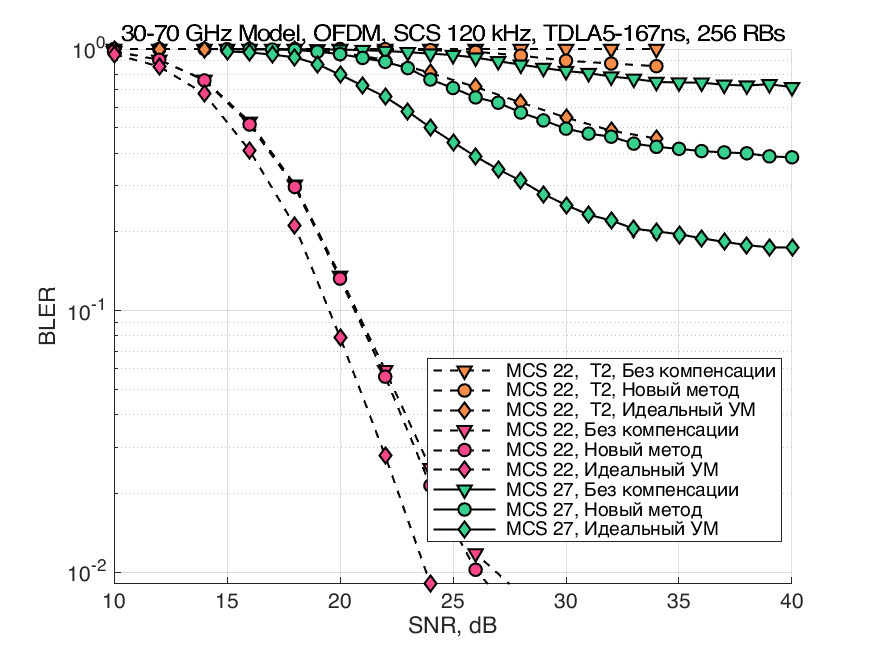
\includegraphics[width=0.49\linewidth]{figs/res/ofdm/OFDM_Nokia_SCS120_MCS22_27.png}
    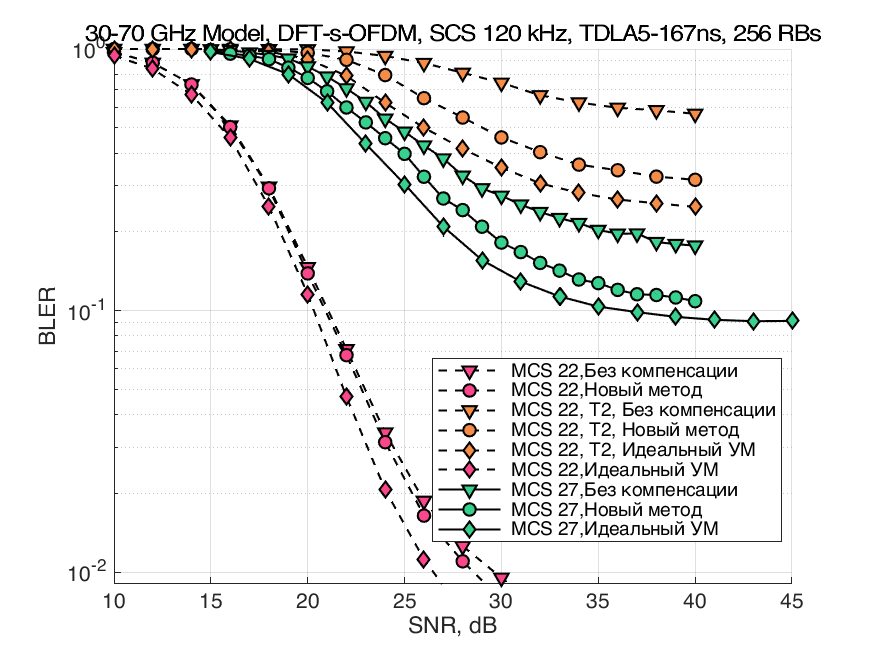
\includegraphics[width=0.49\linewidth]{figs/res/dftsofdm/DFT-s-OFDM_Nokia_SCS120_MCS22_27.png}
    \caption{BLER для SCS 120 кГц, 64-QAM/256 QAM для OFDM (слева) для DFT-s-OFDM(справа)}
    \label{fig:res3070_scs120}
\end{figure}

\begin{figure}[h!]
    \centering
    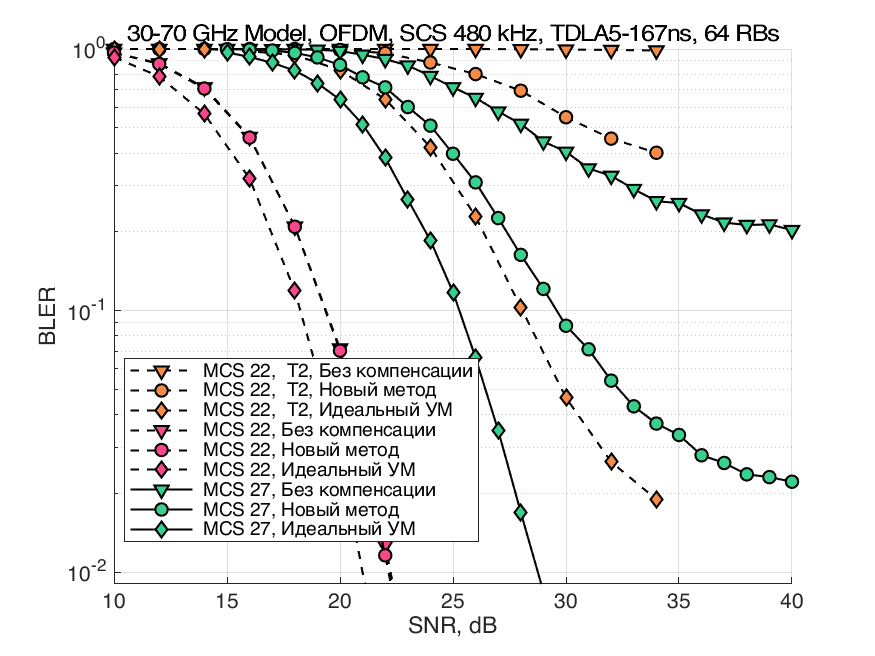
\includegraphics[width=0.49\linewidth]{figs/res/ofdm/OFDM_Nokia_SCS480_MCS22_27.png}
    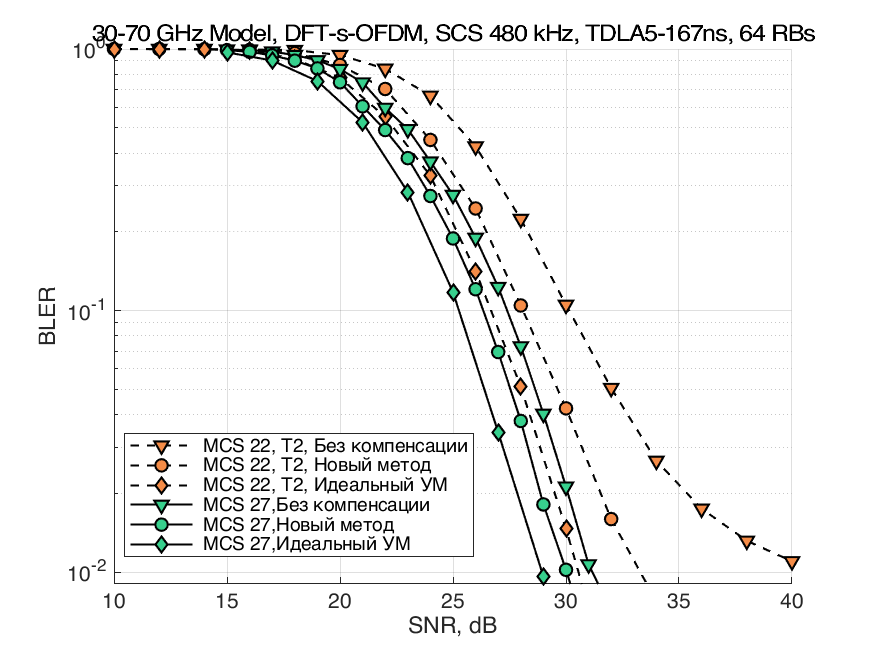
\includegraphics[width=0.49\linewidth]{figs/res/dftsofdm/DFT-s-OFDM_Nokia_SCS480_MCS22_27.png}
    \caption{BLER для SCS 480 кГц, 64-QAM/256 QAM для OFDM (слева) для DFT-s-OFDM(справа)}
    \label{fig:res3070_scs480}
\end{figure}

\begin{figure}[h!]
    \centering
    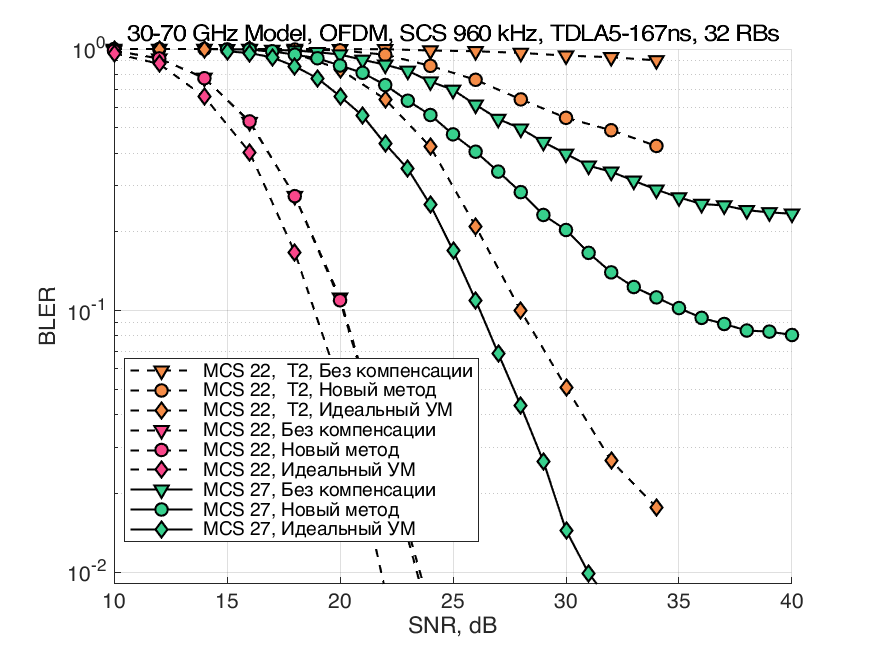
\includegraphics[width=0.49\linewidth]{figs/res/ofdm/OFDM_Nokia_SCS960_MCS22_27.png}
    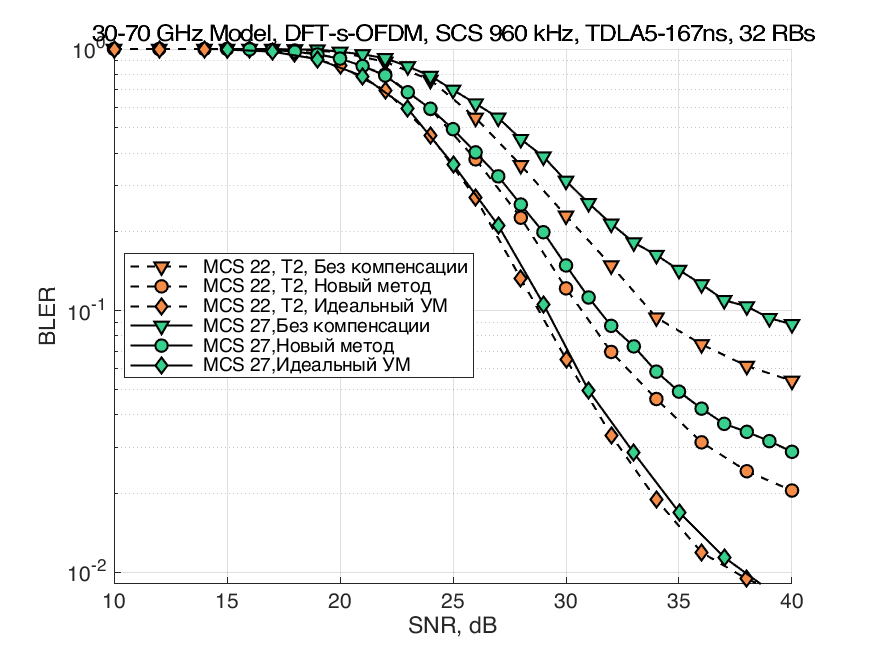
\includegraphics[width=0.49\linewidth]{figs/res/dftsofdm/DFT-s-OFDM_Nokia_SCS960_MCS22_27.png}
    \caption{BLER для SCS 960 кГц, 64-QAM/256 QAM для OFDM (слева) для DFT-s-OFDM(справа)}
    \label{fig:res3070_scs960}
\end{figure}

Кратко опишем полученные результаты. Как и ожидалось, при добавлении
нелинейности УМ в работу LLS, кривая зависимости BLER от SNR стала выше.
Это значит что при том же уровне SNR, количество блоковых ошибок
увеличилось. Например, на рис. \ref{fig:res3070_scs480}(справа)
BLER при SNR$=25$ dB для MCS 27 в случае идеального УМ составлял
$BLER\simeq 10^{-1}$. При добавлении нелинейности УМ, BLER вырос до
$\simeq 3\cdot10^{-1}$. При использовании нового метода компенсации, BLER
понизился до $\simeq 2\cdot10^{-1}$.

Для модели УМ в диапазоне 30-70 ГГц (подходящего для диапазона FR2)
улучшение наблюдается в основном только для модуляций высокого порядка и
при высоких значениях SCS. В частности, для SCS 120 кГц (рис.
\ref{fig:res3070_scs120}), отрицательные эффекты присутствующего в LLS
фазового шума настолько значительны, что при таких искажениях результаты
компенсации нелинейности УМ практически не играют роли. Для высоких
модуляций уровень BLER выравнивается не достигнув значения $10^{-1}$, что
означает плохую производительность системы в целом. Однако даже в таких
условиях можно наблюдать улучшение результатов - кривые BLER в случае
компенсации смещаются на несколько dB по сравнению с случаем отсутствия
компенсации.

Для SCS 480 и 960 кГц (рис. \ref{fig:res3070_scs480},
\ref{fig:res3070_scs960}), в которых возможна более эффективная компенсация
фазового шума, в определенный момент влияние нелинейности УМ становится
основным ограничивающим фактором. В этом случае компенсация нелинейности УМ
может улучшить результат на несколько dB.

\subsection{Результаты симуляций для модели 100-200 ГГц}
В данной секции приведены результаты моделирования для модели УМ 100-200 ГГц. 
На рис. \ref{fig:res100200_scs120} - \ref{fig:res100200_scs960} приведены
зависимости BLER от SNR для различных значений SCS и MCS.
\begin{figure}[h!]
    \centering
    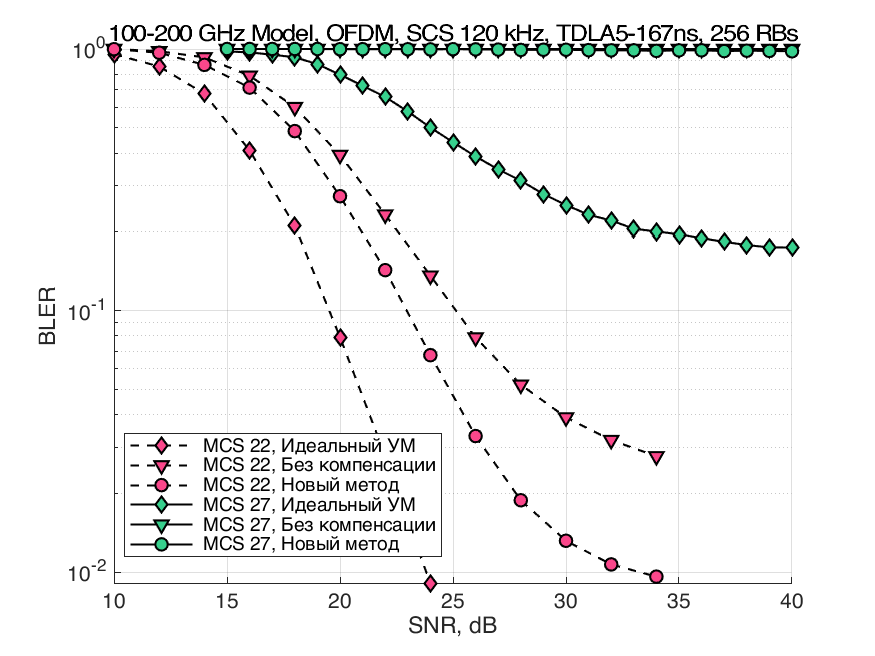
\includegraphics[width=0.49\linewidth]{figs/res/ofdm/OFDM_SubTHz_SCS120_MCS22_27.png}
    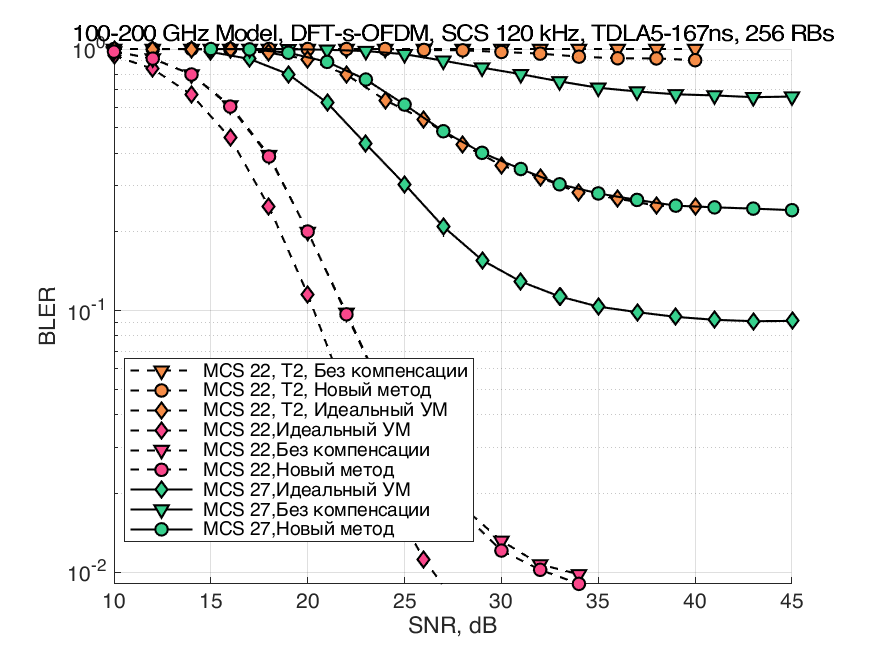
\includegraphics[width=0.49\linewidth]{figs/res/dftsofdm/DFT-s-OFDM_SubTHz_SCS120_MCS22_27.png}
    \caption{BLER для SCS 120 кГц, 64-QAM/256 QAM для OFDM (слева) для DFT-s-OFDM(справа)}
    \label{fig:res100200_scs120}
\end{figure}

\begin{figure}[h!]
    \centering
    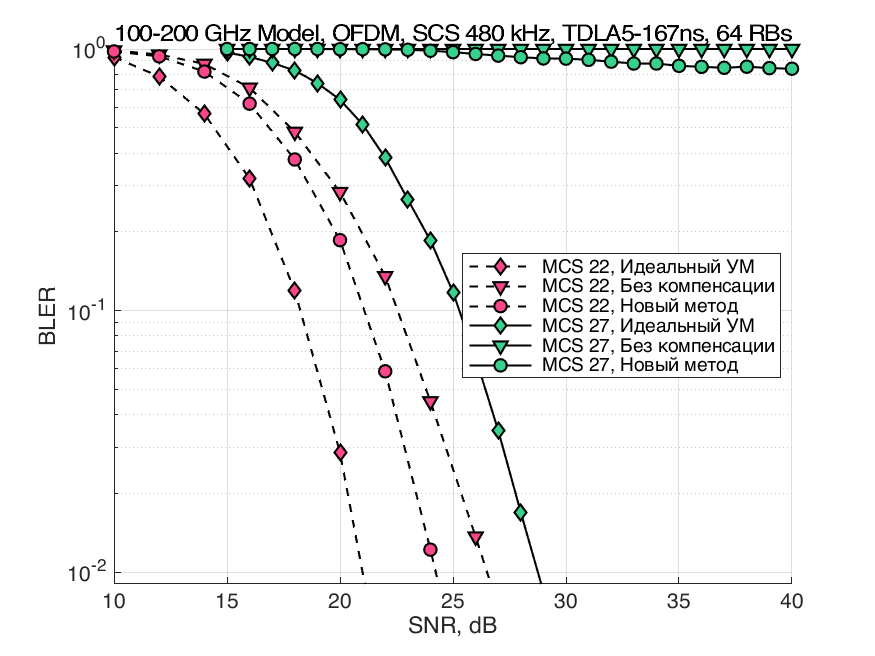
\includegraphics[width=0.49\linewidth]{figs/res/ofdm/OFDM_SubTHz_SCS480_MCS22_27.png}
    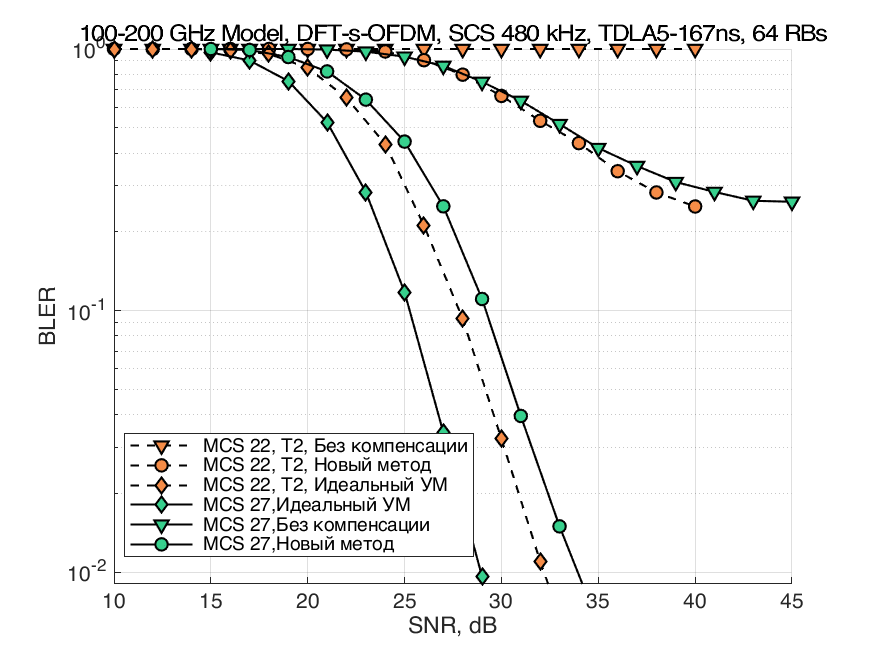
\includegraphics[width=0.49\linewidth]{figs/res/dftsofdm/DFT-s-OFDM_SubTHz_SCS480_MCS22_27.png}
    \caption{BLER для SCS 480 кГц, 64-QAM/256 QAM для OFDM (слева) для DFT-s-OFDM(справа)}
    \label{fig:res100200_scs480}
\end{figure}

\begin{figure}[h!]
    \centering
    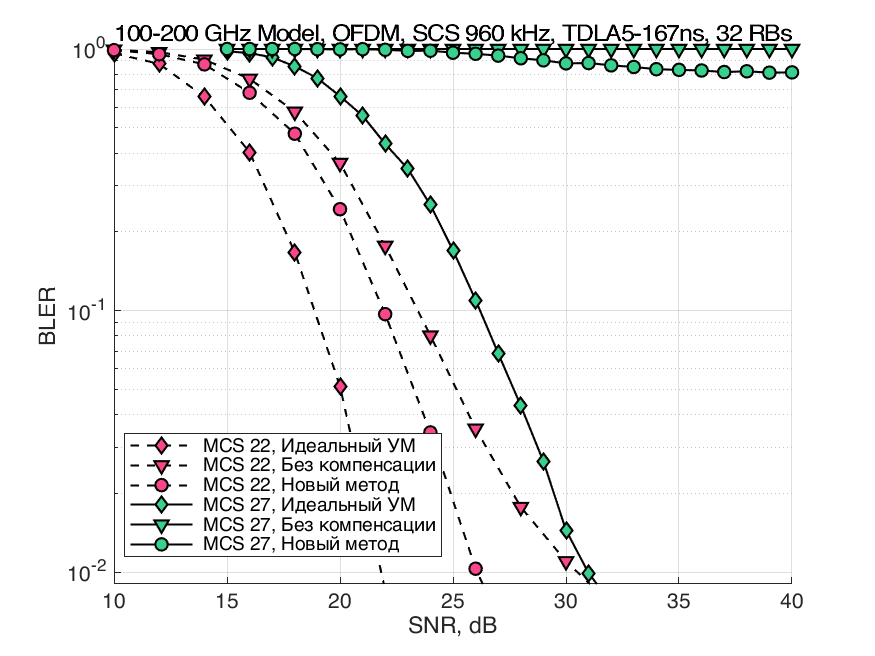
\includegraphics[width=0.49\linewidth]{figs/res/ofdm/OFDM_SubTHz_SCS960_MCS22_27.png}
    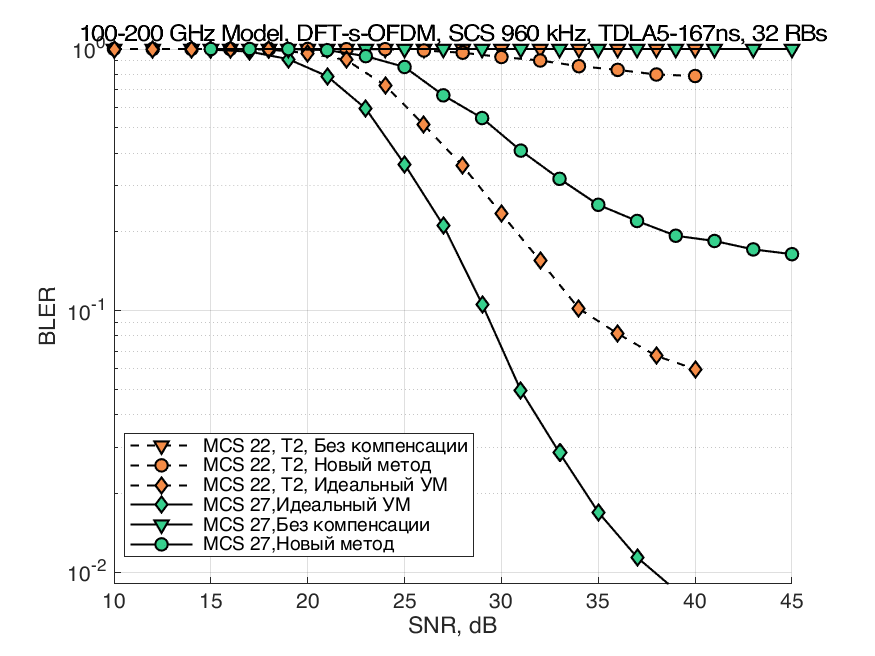
\includegraphics[width=0.49\linewidth]{figs/res/dftsofdm/DFT-s-OFDM_SubTHz_SCS960_MCS22_27.png}
    \caption{BLER для SCS 960 кГц, 64-QAM/256 QAM для OFDM (слева) для DFT-s-OFDM(справа)}
    \label{fig:res100200_scs960}
\end{figure}
Для модели 100-200 ГГц, влияние нелинейности УМ увеличивается, и в
большинстве случаев превосходит влияние фазовых шумов. Это связано с общим
ухудшением характирестик УМ в данном диапазоне, из-за чего происходят более
значительные искажения. В некоторых случаях, искажения настолько сильные,
что получение какой-либо информации практически невозможно, будь то с
компенсацией или без. Предложенный метод компенсации демонстрирует
улучшение результата для MCS 22 и выше.


% Не смотря на возможность различных имплементаций, диктуемая логикой
% последовательность компенсации искажений в порядке, обратному их появлению
% в системе оказывается оптимальным. Таким образом, искажения должны быть
% компенсированы в порядке канал, усилитель мощности, фазовые шумы.  
% TBD

